\documentclass[a4paper,12pt]{article}
\usepackage[margin=18mm]{geometry}
\usepackage{tikz}
\usepackage{amsmath}
\usepackage{xcolor}
\newcommand{\pFourCell}[2]{\makebox[#1em][c]{\ensuremath{#2}}}
\newcommand{\pFourCenterBox}[1]{\begingroup\setbox0=\hbox{$\displaystyle #1$}\dimen0=\ht0\advance\dimen0 by -\dp0\divide\dimen0 by 2\lower\dimen0\box0\endgroup}
\newdimen\pFourFractionRuleThickness
\pFourFractionRuleThickness=0.4pt
\newcommand{\pFourTopAlign}[3]{\raisebox{-#1}[0pt][\dimexpr #1 + #2\relax]{\ensuremath{\displaystyle #3}}}
\newcommand{\pFourBottomAlign}[3]{\raisebox{#2}[\dimexpr #1 + #2\relax][0pt]{\ensuremath{\displaystyle #3}}}
\newcommand{\pFourFractionInner}[2]{\hbox to #1{\hss$\displaystyle #2$\hss}}
\newcommand{\pFourFractionC}[4]{\begingroup\color{#1}\genfrac{}{}{\pFourFractionRuleThickness}{0}{\raisebox{0.14em}{\pFourFractionInner{#2}{{\color{black}#3}}}}{\raisebox{-0.18em}{\pFourFractionInner{#2}{{\color{black}#4}}}}\endgroup}
\newcommand{\pFourFraction}[3]{\genfrac{}{}{\pFourFractionRuleThickness}{0}{\raisebox{0.14em}{\pFourFractionInner{#1}{#2}}}{\raisebox{-0.18em}{\pFourFractionInner{#1}{#3}}}}
\newcommand{\pFourRootC}[2]{\begingroup\setbox0=\hbox{$\displaystyle #2$}\setbox2=\hbox{$\displaystyle \sqrt{\phantom{\copy0}}$}\dimen0=\wd2\advance\dimen0 by -\wd0\hbox{\rlap{\textcolor{#1}{\copy2}}\kern\dimen0\box0}\endgroup}
\newcommand{\pFourRoot}[1]{\pFourRootC{black}{#1}}
\newcommand{\pFourRootDegreeC}[3]{\begingroup\setbox0=\hbox{$\displaystyle #3$}\setbox2=\hbox{$\displaystyle \sqrt[#2]{\phantom{\copy0}}$}\dimen0=\wd2\advance\dimen0 by -\wd0\hbox{\rlap{\textcolor{#1}{\copy2}}\kern\dimen0\box0}\endgroup}
\newcommand{\pFourRootDegree}[2]{\pFourRootDegreeC{black}{#1}{#2}}
\pagestyle{empty}
\begin{document}

\section*{Spaltentreue LaTeX-Ausgabe}
\noindent Gleichung: \texttt{a}\texttt{/}\texttt{sin}\texttt{(}\ensuremath{\alpha}\texttt{)=}\texttt{b}\texttt{/}\texttt{sin}\texttt{(}\ensuremath{\beta}\texttt{)} \hfill Zielvariable: \ensuremath{\alpha} \hfill Profil: \texttt{standard}

\vspace{8mm}
\begin{center}
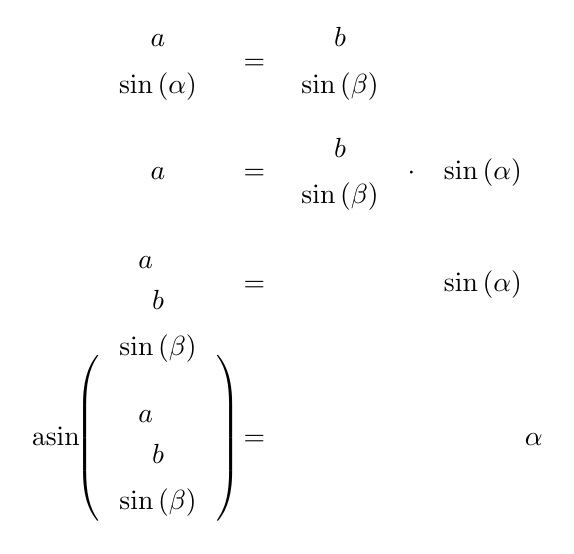
\begin{tikzpicture}[x=1em,y=-1em]
\node[anchor=base, inner sep=0pt] at (4.71,2.7) {$\pFourFraction{4.58em}{\makebox[4.58em][c]{\ensuremath{\pFourCell{0.9}{a}}}}{\pFourCell{4.58}{\sin\left(\alpha\right)}}$};
\node[anchor=base, inner sep=0pt] at (11.29,2.7) {$\pFourFraction{4.58em}{\makebox[4.58em][c]{\ensuremath{\pFourCell{0.9}{b}}}}{\pFourCell{4.58}{\sin\left(\beta\right)}}$};
\node[anchor=base, inner sep=0pt] at (8.19,2.7) {$\pFourCell{1.62}{=}$};
\node[anchor=base, inner sep=0pt] at (11.29,6.69) {$\pFourFraction{4.58em}{\makebox[4.58em][c]{\ensuremath{\pFourCell{0.9}{b}}}}{\pFourCell{4.58}{\sin\left(\beta\right)}}$};
\node[anchor=base, inner sep=0pt] at (4.71,6.69) {$a$};
\node[anchor=base, inner sep=0pt] at (8.19,6.69) {$\pFourCell{1.62}{=}$};
\node[anchor=base, inner sep=0pt] at (13.87,6.69) {$\pFourCell{0.58}{\cdot{}}$};
\node[anchor=base, inner sep=0pt] at (16.45,6.69) {$\pFourCell{4.58}{\sin\left(\alpha\right)}$};
\node[anchor=base, inner sep=0pt] at (4.71,10.72) {$\pFourFraction{4.58em}{\pFourCell{3.68}{a}\pFourCell{0}{}\pFourCell{0.9}{}\pFourCell{0}{}}{\pFourTopAlign{0.6em}{0.36em}{\pFourFraction{4.58em}{\makebox[4.58em][c]{\ensuremath{\pFourCell{0.9}{b}}}}{\pFourCell{4.58}{\sin\left(\beta\right)}}}}$};
\node[anchor=base, inner sep=0pt] at (8.19,10.72) {$\pFourCell{1.62}{=}$};
\node[anchor=base, inner sep=0pt] at (16.45,10.72) {$\pFourCell{4.58}{\sin\left(\alpha\right)}$};
\node[anchor=base, inner sep=0pt] at (4.71,16.28) {$\pFourFraction{4.58em}{\pFourCell{3.68}{a}\pFourCell{0}{}\pFourCell{0.9}{}\pFourCell{0}{}}{\pFourTopAlign{0.6em}{0.36em}{\pFourFraction{4.58em}{\makebox[4.58em][c]{\ensuremath{\pFourCell{0.9}{b}}}}{\pFourCell{4.58}{\sin\left(\beta\right)}}}}$};
\node[anchor=base, inner sep=0pt] at (1.02,16.28) {$\pFourCell{2.04}{\operatorname{asin}}$};
\node[anchor=base, inner sep=0pt] at (2.23,16.28) {$\pFourCell{0.38}{\left(\raisebox{0pt}[1.6em][2.92em]{\rule{0pt}{0pt}}\right.}$};
\node[anchor=base, inner sep=0pt] at (7.19,16.28) {$\pFourCell{0.38}{\left.\raisebox{0pt}[1.6em][2.92em]{\rule{0pt}{0pt}}\right)}$};
\node[anchor=base, inner sep=0pt] at (8.19,16.28) {$\pFourCell{1.62}{=}$};
\node[anchor=base, inner sep=0pt] at (18.29,16.28) {$\pFourCell{0.9}{\alpha}$};
\end{tikzpicture}
\end{center}


\newpage
\section*{Spaltentreue LaTeX-Ausgabe mit Spaltengrenzen}
\vspace{6mm}
\begin{center}
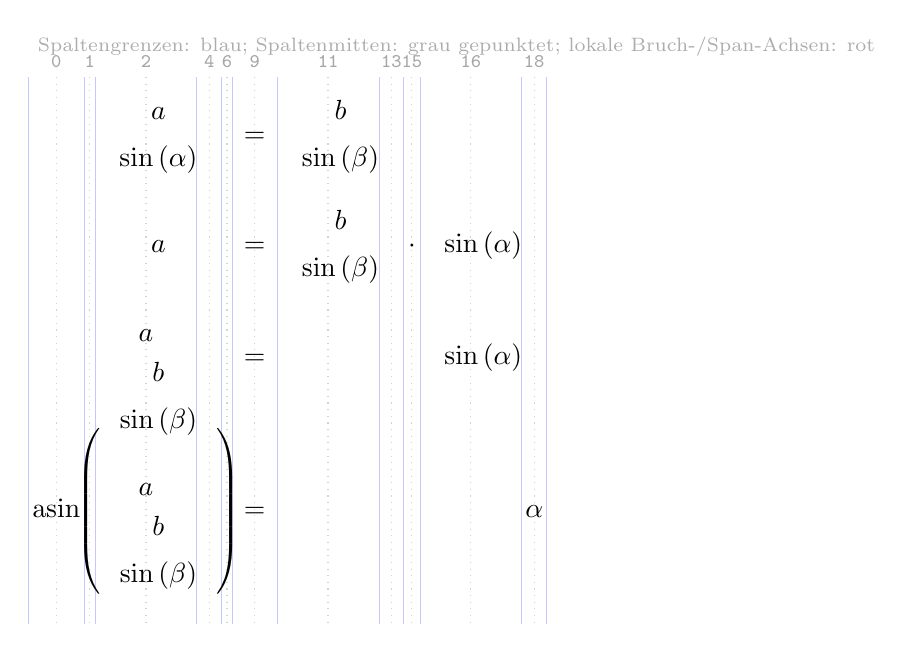
\begin{tikzpicture}[x=1em,y=-1em]
\node[font={\scriptsize}, text=gray!65, anchor=west] at (0,-0.75) {Spaltengrenzen: blau; Spaltenmitten: grau gepunktet; lokale Bruch-/Span-Achsen: rot};
\draw[blue!22, line width=0.28pt] (0,0.35) -- (0,20.1);
\draw[blue!22, line width=0.28pt] (2.04,0.35) -- (2.04,20.1);
\draw[blue!22, line width=0.28pt] (2.42,0.35) -- (2.42,20.1);
\draw[blue!22, line width=0.28pt] (6.1,0.35) -- (6.1,20.1);
\draw[blue!22, line width=0.28pt] (7,0.35) -- (7,20.1);
\draw[blue!22, line width=0.28pt] (7.38,0.35) -- (7.38,20.1);
\draw[blue!22, line width=0.28pt] (9,0.35) -- (9,20.1);
\draw[blue!22, line width=0.28pt] (12.68,0.35) -- (12.68,20.1);
\draw[blue!22, line width=0.28pt] (13.58,0.35) -- (13.58,20.1);
\draw[blue!22, line width=0.28pt] (14.16,0.35) -- (14.16,20.1);
\draw[blue!22, line width=0.28pt] (17.84,0.35) -- (17.84,20.1);
\draw[blue!22, line width=0.28pt] (18.74,0.35) -- (18.74,20.1);
\draw[gray!35, dotted] (1.02,0.35) -- (1.02,20.1);
\node[font={\ttfamily\scriptsize}, text=gray!70, anchor=base] at (1.02,0) {0};
\draw[gray!35, dotted] (2.23,0.35) -- (2.23,20.1);
\node[font={\ttfamily\scriptsize}, text=gray!70, anchor=base] at (2.23,0) {1};
\draw[gray!35, dotted] (4.26,0.35) -- (4.26,20.1);
\node[font={\ttfamily\scriptsize}, text=gray!70, anchor=base] at (4.26,0) {2};
\draw[gray!35, dotted] (6.55,0.35) -- (6.55,20.1);
\node[font={\ttfamily\scriptsize}, text=gray!70, anchor=base] at (6.55,0) {4};
\draw[gray!35, dotted] (7.19,0.35) -- (7.19,20.1);
\node[font={\ttfamily\scriptsize}, text=gray!70, anchor=base] at (7.19,0) {6};
\draw[gray!35, dotted] (8.19,0.35) -- (8.19,20.1);
\node[font={\ttfamily\scriptsize}, text=gray!70, anchor=base] at (8.19,0) {9};
\draw[gray!35, dotted] (10.84,0.35) -- (10.84,20.1);
\node[font={\ttfamily\scriptsize}, text=gray!70, anchor=base] at (10.84,0) {11};
\draw[gray!35, dotted] (13.13,0.35) -- (13.13,20.1);
\node[font={\ttfamily\scriptsize}, text=gray!70, anchor=base] at (13.13,0) {13};
\draw[gray!35, dotted] (13.87,0.35) -- (13.87,20.1);
\node[font={\ttfamily\scriptsize}, text=gray!70, anchor=base] at (13.87,0) {15};
\draw[gray!35, dotted] (16,0.35) -- (16,20.1);
\node[font={\ttfamily\scriptsize}, text=gray!70, anchor=base] at (16,0) {16};
\draw[gray!35, dotted] (18.29,0.35) -- (18.29,20.1);
\node[font={\ttfamily\scriptsize}, text=gray!70, anchor=base] at (18.29,0) {18};
\node[anchor=base, inner sep=0pt] at (4.71,2.7) {$\pFourFraction{4.58em}{\makebox[4.58em][c]{\ensuremath{\pFourCell{0.9}{a}}}}{\pFourCell{4.58}{\sin\left(\alpha\right)}}$};
\node[anchor=base, inner sep=0pt] at (11.29,2.7) {$\pFourFraction{4.58em}{\makebox[4.58em][c]{\ensuremath{\pFourCell{0.9}{b}}}}{\pFourCell{4.58}{\sin\left(\beta\right)}}$};
\node[anchor=base, inner sep=0pt] at (8.19,2.7) {$\pFourCell{1.62}{=}$};
\node[anchor=base, inner sep=0pt] at (11.29,6.69) {$\pFourFraction{4.58em}{\makebox[4.58em][c]{\ensuremath{\pFourCell{0.9}{b}}}}{\pFourCell{4.58}{\sin\left(\beta\right)}}$};
\node[anchor=base, inner sep=0pt] at (4.71,6.69) {$a$};
\node[anchor=base, inner sep=0pt] at (8.19,6.69) {$\pFourCell{1.62}{=}$};
\node[anchor=base, inner sep=0pt] at (13.87,6.69) {$\pFourCell{0.58}{\cdot{}}$};
\node[anchor=base, inner sep=0pt] at (16.45,6.69) {$\pFourCell{4.58}{\sin\left(\alpha\right)}$};
\node[anchor=base, inner sep=0pt] at (4.71,10.72) {$\pFourFraction{4.58em}{\pFourCell{3.68}{a}\pFourCell{0}{}\pFourCell{0.9}{}\pFourCell{0}{}}{\pFourTopAlign{0.6em}{0.36em}{\pFourFraction{4.58em}{\makebox[4.58em][c]{\ensuremath{\pFourCell{0.9}{b}}}}{\pFourCell{4.58}{\sin\left(\beta\right)}}}}$};
\node[anchor=base, inner sep=0pt] at (8.19,10.72) {$\pFourCell{1.62}{=}$};
\node[anchor=base, inner sep=0pt] at (16.45,10.72) {$\pFourCell{4.58}{\sin\left(\alpha\right)}$};
\node[anchor=base, inner sep=0pt] at (4.71,16.28) {$\pFourFraction{4.58em}{\pFourCell{3.68}{a}\pFourCell{0}{}\pFourCell{0.9}{}\pFourCell{0}{}}{\pFourTopAlign{0.6em}{0.36em}{\pFourFraction{4.58em}{\makebox[4.58em][c]{\ensuremath{\pFourCell{0.9}{b}}}}{\pFourCell{4.58}{\sin\left(\beta\right)}}}}$};
\node[anchor=base, inner sep=0pt] at (1.02,16.28) {$\pFourCell{2.04}{\operatorname{asin}}$};
\node[anchor=base, inner sep=0pt] at (2.23,16.28) {$\pFourCell{0.38}{\left(\raisebox{0pt}[1.6em][2.92em]{\rule{0pt}{0pt}}\right.}$};
\node[anchor=base, inner sep=0pt] at (7.19,16.28) {$\pFourCell{0.38}{\left.\raisebox{0pt}[1.6em][2.92em]{\rule{0pt}{0pt}}\right)}$};
\node[anchor=base, inner sep=0pt] at (8.19,16.28) {$\pFourCell{1.62}{=}$};
\node[anchor=base, inner sep=0pt] at (18.29,16.28) {$\pFourCell{0.9}{\alpha}$};
\end{tikzpicture}
\end{center}
\end{document}
